%!TEX root = ../report.tex
\chapter{Technology Stack}\label{ch:technology-stack}
Finding the right technology stack for a project is a major part of the overall process of realizing a project.
Multiple considerations should be taken into account which we will cover in this section.
This section is a detailed view on the technology stack we have utilized in the project and why we used it.

\section{Keep it simple and agile}\label{sec:keep-it-simple-and-agile}

Finding a proper technology stack starts with deciding a fitting solution for the actual context in which the project
should be realized.
As the project will be developed in a short-term project of 5 months within \ac{sofa} at Fontys Venlo we
had to go with an agile as well as easy to start with technology.
This enables all team members to get started quickly as well as to adapt accordingly if something does not work out as
planned.

We started with a small concept, and some sketches of how the product could look like.
The actual set of features was not fixed at this point in time.
We knew that the project scope would change during the project phase.
That's why it is even more important to choose for an agile approach.

\section{Project requirements}\label{sec:project-requirements}

As the project is focussing on secure as well as fast communication between several users across the internet, we wanted
to choose a technology stack that supports various system platforms as well as easy migration possibilities for a later
stage of the project.
This would allow us to adapt our developed parts to be translated to further platforms and devices.
As more than 60\% of all users are accessing the internet via mobile devices the focus should also lie on technologies
which are fully supported by mobile platforms.
So we can easily port the logic to a mobile client as we only have to adapt the \ac{ui} later on.

As security and privacy are our core principles we needed to take this into consideration for our technology stack.
Our focus was set to various technologies which have been around for quite some time already, so we can be sure that
major security vulnerabilities have been eliminated beforehand.

\section{Open-source technologies}\label{sec:open-source-technologies}

Going with open-source technologies provides multiple benefits.
First, it enables to project team to focus on the business part of the application.
Most of the time, there is already a good open-source solution for general tasks like frontend frameworks, database
systems or encryption algorithms.
Those implementations enable the team to safe a lot of time as the components do not have to be developed by ourselves.
Last but not least are those already implemented solutions more secure as more people have their eyes on it and report
and fix bugs.

\section{Ecosystem}\label{sec:ecosystem}

As a result of the larger community of open-source technologies a better ecosystem will go along with it.
Important for using open-source software is, that it is properly documented and that is already known in the community.
This helps with later bug fixing and solution finding.
The more people using a technology the more questions and answers will be available on sites like Stackoverflow or
GitHub forums.

Furthermore, there will be more third-party components and solutions available
(for example via npm (node package manager)).

\section{Long-term trends and support}\label{sec:long-term-trends-and-support}

Lastly, a detailed look on the long-term development of available technologies should be considered.
As said before, we should aim for mature technologies as they are more robust, reliable and most of the time also more
secure which is crucial for this project specifically.

\section{Final technology stack}\label{sec:final-technology-stack}

Taking all the above listed considerations into account we have come up with the following technology stack for our
\ac{sofa} project:

\subsection{Frontend}\label{subsec:frontend}

\begin{itemize}
    \item \textbf{Electron:} We decided to go with Electron as it enables us to develop one solution which can be
        deployed across several platforms including Windows, macOS, and Linux.
        As Electron is not that difficult to include into a default setup we decided to utilize the technology as this
        increases the target group significantly.
    \item \textbf{Angular:} We decided to go with Angular as major frontend framework.
        It enables us to handle data efficiently between several components.
        Furthermore, it comes with useful features, for example to dynamically re-render views if the displayed data
        changes.
        Additionally, it is compatible with multiple mobile application frameworks like NativeScript.
    \item \textbf{Angular Material:} Angular Material provides us with a comprehensive \ac{ui} library.
        The library ships with preconfigured elements such as buttons, menus, navigation options, form fields and many
        more.
    \item \textbf{SCSS:} To complete our frontend stack we utilize SCSS. It provides additional functionality to
        standard CSS like variables, nested operations, and it makes it possible to dynamically render themes for
        Angular Material.
    \item \textbf{NPM:} Is a package manager for \hyperref[subsec:backend]{\textbf{Node.js.}}.
        NPM gives us access to many useful open source modules.
        In many cases, this saves us from writing code for well-known use cases for which there are already many
        solutions.
    \item \textbf{Prisma client:} During development of the settings service, we found the prisma client library.
        This client functions on the database access layer and makes writing queries easier.
        Setting up the client was very simple thanks to the excellent documentation of the library provider.
        We kept using this library for the first few weeks of implementation phase, however, it turned out that the
        client did not support some very important functions of MySQL.
        We noticed this while trying to write a query with the \enquote{LIKE} keyword, which was not available in the
        client.
        As this made implementation of the query using the client very difficult, it was decided to switch the MySQL
        client and use the more straight forward \enquote{mysql2} client provided by MySQL, which was also used in the
        existing services.
        Currently, the prisma service is still being used for simple queries in the
        \hyperref[subsubsec:settingsSer]{settings service}.
        However, it is planned to replace these queries with the mysql2 client later on, to have the same standard
        everywhere.
        For time reasons this has not been finished yet.
\end{itemize}

\subsubsection{Angular}

\paragraph{Introduction to Frameworks}
First, it should be clarified what a framework is.
A framework gives the developer an environment for his application programming.
Unlike a library, a framework does not represent a stand-alone program, but serves as a set of guidelines to assist the
developer in generating code.
A framework assumes that the developer writes his code according to some rules and in a certain structure.
The big advantage is that a uniform structure is always kept.
A further advantage of Frameworks is the frequent integration of libraries.
Libraries provide one with a set of pre-built elements that the developer can reuse anywhere in the code without having
to rewrite them every time.

\paragraph{Functionality of a Script-Language}
Angular works with TypeScript, a scripting language developed in 2012 by Microsoft employee and designer of the C
language, Anders Hejlsberg.
The developed TypeScript compiler compiles TypeScript code to plain JavaScript code according to ECMA Script 3.
Therefore, any JavaScript code represents valid TypeScript code.
Unlike JavaScript, TypeScript has language constructs such as classes, inheritance and, most importantly, strong static
typing.
A scripting language differs from a classical programming language in that it is not compiled once by a compiler in
order to be executed, but by the browser's interpreter each time it is executed.
Unlike PHP, the JavaScript generated by the TypeScript compiler is not executed on the server side but on the client
side by the browser.
This allows the creation of dynamic web pages that can adapt to the user.
JavaScripts are able to register user input and can directly manipulate displayed HTML documents and thus change the
display and content of the elements without first having to send a request to the server.
All changes do not take place on the server side, but locally in the browser.
This capacity of JavaScript enables the creation of interactive and dynamic web pages.
As before, what is seen in the browser is an HTML document, where the various HTML elements are designed with the help
of CSS.
The client does not retrieve the JavaScript directly from the server, but an HTML document in which JavaScript can be
included.
If this is the case, the client side requests the JavaScript in another request to the server and then executes it in
the browser.
This script then has access to the previously requested HTML document and can control and modify individual elements
via the Document Object Model (DOM).

\paragraph{SocialStuff is a Single Page Application}
The frontend for SocialStuff, uses Angular not only in parts of the project, but is built entirely on Angular.
The project can be seen as a \enquote{single page application}.
This means that an HTTP request is sent only once when the page is called.
The received HTML document contains the JavaScript code to dynamically adjust the content of the page in the browser.
Only endpoints are called via a server to receive JSON files and to be able to display different content.
This allows for much better usability.
Even though this model is called Single Page Application, it is still possible to access different pages within the
website via the URL. The difference to a classic dynamic website (e.g. using PHP) is that a new HTML document does not
have to be requested from the server for each page that is accessed, but the HTML document is mutated locally so that
it only appears to be new HTML document.

\begin{figure}[H]
    \centering
    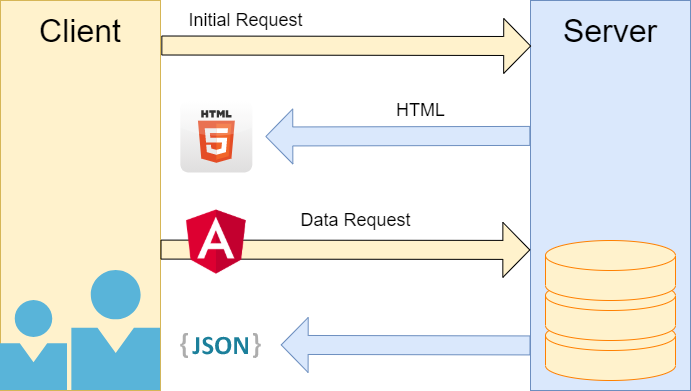
\includegraphics[width=1.0\textwidth]{./images/single_page_app}
    \caption{Single Page Application}
    \label{fig:singpageapp}
\end{figure}

\newpage
\paragraph{Project Structure in Angular}
In this part, the design and structure of an Angular project will be discussed in order to explain the basics of this
framework.
For the sake of simplicity, a simple Hello World project was created for this part, consisting of a home page displaying
a Hello World logo and a welcome text and sample about page.

\begin{figure}[H]
    \centering
    \fbox{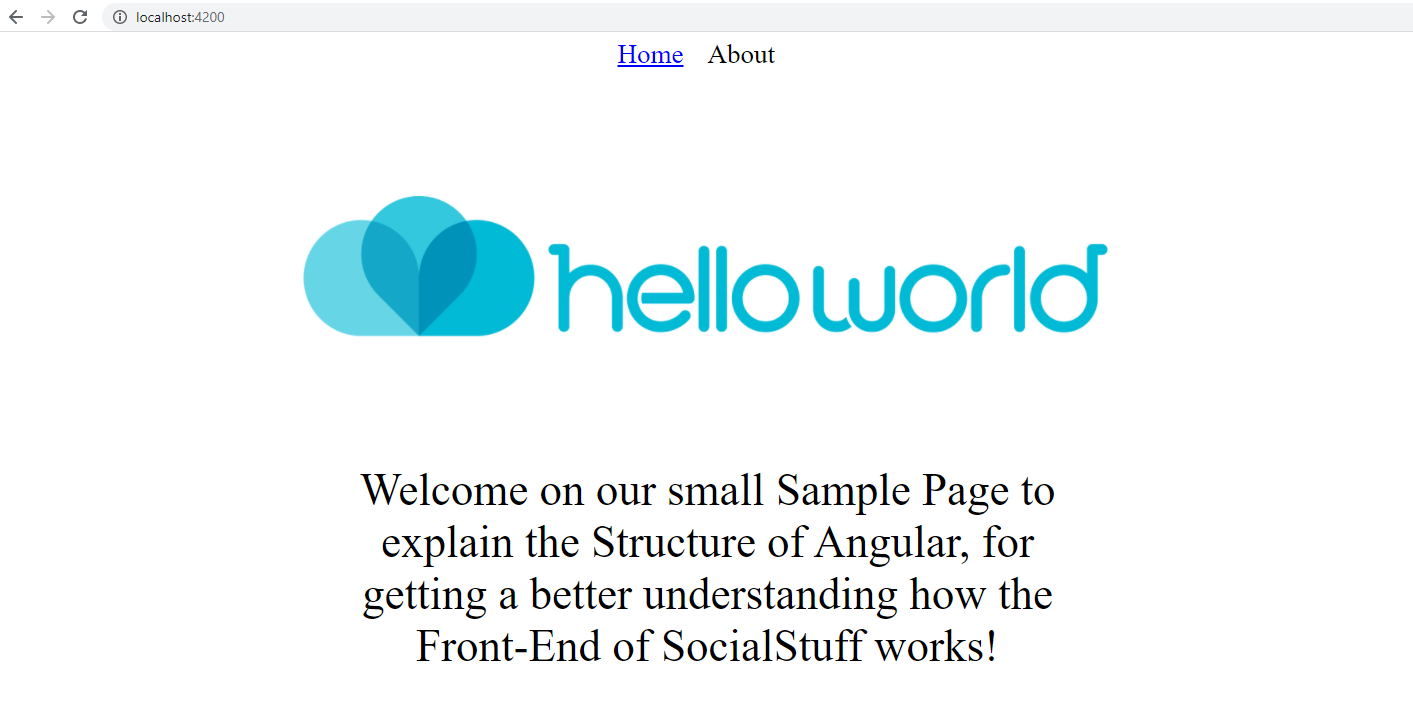
\includegraphics[width=1.0\textwidth]{./images/SamplePage_Home}}
    \caption{Homepage Example Website}
    \label{fig:examplehomepage}
\end{figure}

\begin{figure}[H]
    \centering
    \fbox{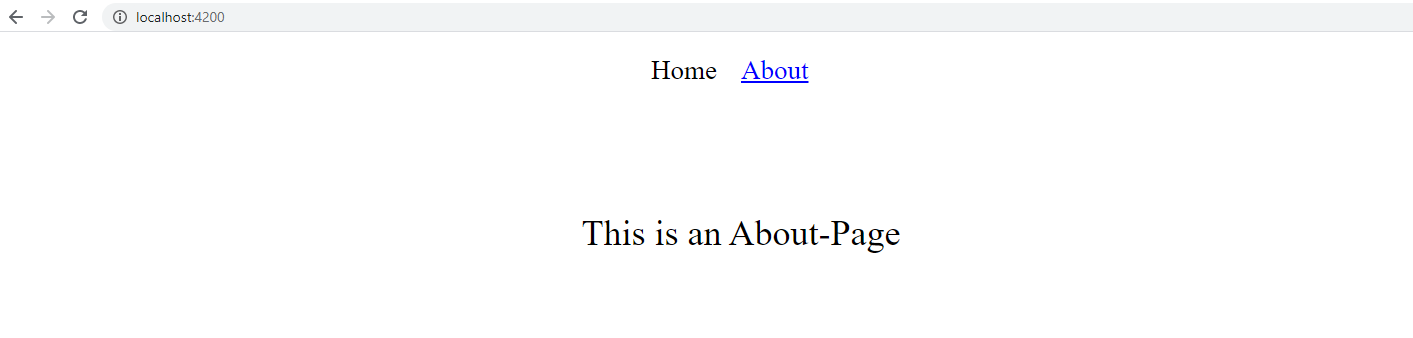
\includegraphics[width=1.0\textwidth]{./images/SamplePage_About}}
    \caption{About Example Website}
    \label{fig:figure41}
\end{figure}

\newpage
\begin{figure}[H]
    \centering
    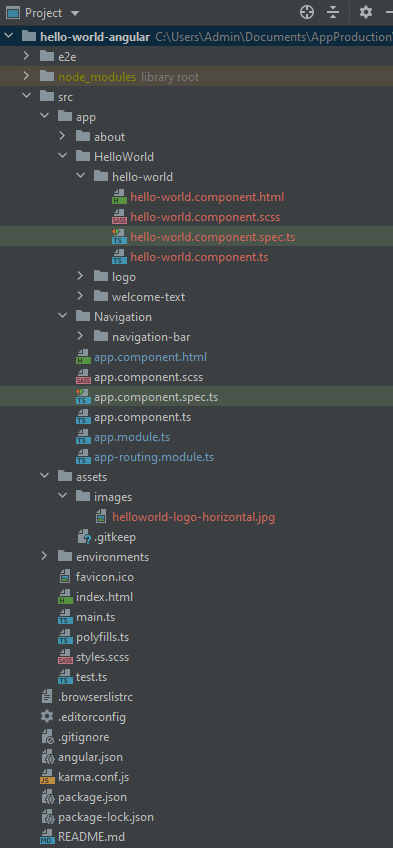
\includegraphics[height=0.5\textheight]{./images/SamplePage_ProjectStructure}
    \caption{Project Structure}
    \label{fig:figure42}
\end{figure}
\newline

Angular projects always resemble each other in their layout since the basic structure is predefined by the
initialization of a new project via the webpack template (Figure 6).
If you look at the structure and names of the folders, you can already find parts of the website, at least from the
naming. \\
All visible elements of the web page are divided into components.
A component consists of four files (seeing folder HelloWorld/hello-world):

\begin{enumerate}
    \item An HTML-file presenting the structure of the component
    \item A scss-file styling the component
    \item A TypeScript-file containing the functionality of the component
    \item A TypeScript-file testing the functionality.
\end{enumerate}

How the files of a component are structured individually will be explained later, first it must be understood what
happens when the web page is called for the first time via a URL. \\
In the source folder there is a file called \enquote{index.html} this is the only HTML document the server is sending
as a response to the client.

\begin{figure}[H]
    \centering
    \fbox{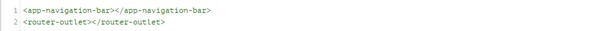
\includegraphics[width=1.0\textwidth]{./images/html_app_root}}
    \caption{HTML of App-Root Component}
    \label{fig:htmlapproot}
\end{figure}

The HTML-File of the App-Root Component only consist of two tags.
The first tag loads the NavigationBar component, the second tag loads the router outlet.
The router outlet loads angular components dynamically, based on the current URL.
Which component should be loaded under which URL is defined in the \enquote{app-routing.module.ts} file.

\begin{figure}[H]
    \centering
    \fbox{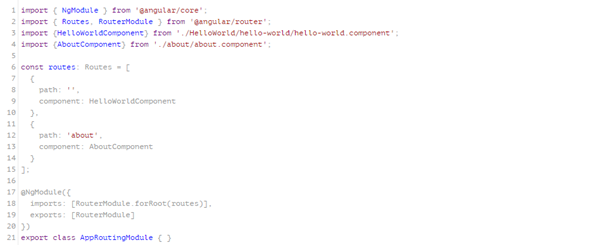
\includegraphics[width=1.0\textwidth]{./images/app_routing_module}}
    \caption{app-routing.module.ts}
    \label{fig:approutingmodule}
\end{figure}

From line 6 - 15 all the routes for this HelloWorld Project are described.
A route always exists of at least a path and a component which should be loaded when the certain path is called.
When first entering the Website without defining a certain path (Figure app-routing.module.ts, l.8) the HelloWorld
component is loaded inside the router outlet (Figure app-routing.module.ts, l.9).
HTML of HelloWorld Component:

\begin{figure}[H]
    \centering
    \fbox{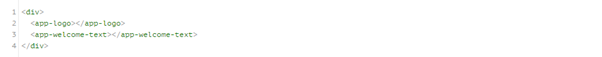
\includegraphics[width=1.0\textwidth]{./images/html_helloworld}}
    \caption{HTML of HelloWorldComponent}
    \label{fig:htmlhello}
\end{figure}

The HelloWorld component is then again calling other components.
Without going into details, this small example shows what component based web frameworks are all about: Splitting up a
website into smaller components, creating clear and reusable code
(more in chapter \hyperref[subsec:components]{\textbf{Components}}).

\subsection{Backend}\label{subsec:backend}

\begin{itemize}
    \item \textbf{NodeJS:} The reason we utilized NodeJS as we wanted to use TypeScript.
        With NodeJS we are able to write code in just one programming language (TypeScript).
        With this approach we can compile the code to plain JavaScript, so we can share code between the frontend and
        backend as well as writing less code overall.
        Node.js is a JavaScript-based application framework, allowing developing fast, scalable network applications.
        At its heart is Google's V8 JavaScript engine, which was originally developed for Chrome.
        The engine increases performance by compiling JavaScript directly into native machine code
        (just-in-time compilation).
        A decisive special feature of the framework is also its ability to communicate with events as well as to
        process multiple client connections simultaneously, which makes Node.js particularly interesting for web server
        development.
        Traditionally, servers are not event-driven, but thread-based.
        The best way to think of it is like the queue in a fast food restaurant: with a thread-based server, you place
        your order and then continue to wait at your place in the queue until your order arrives; during this time,
        however, the queue does not move any further because the waitress does not have the opportunity to serve the
        next customer.
        With an event-driven server, on the other hand, you place your order and then step aside to make room for the
        next customer.
        Meanwhile, your order is processed in the background and brought to you or made available for collection as
        soon as it is ready.
        The crucial point here is that the acceptance of new orders, i.e. the input-output operation of the server,
        is not hindered - this is why we also speak of non-blocking I/O (in contrast to blocking I/O in classic,
        thread-based servers).
        In the case of server requests, it is really only a matter of microseconds - but microseconds are also
        important, especially with highly scalable servers and many simultaneous, data-intensive requests~\cite{nodejs}.
    \item \textbf{Express:} Express is a wrapper around the native \ac{http} module of NodeJS.
        It makes it easier to create routes and middlewares and to compose them together into an application.
    \item \textbf{MongoDB:} We decided to go with MongoDB for the chat service so that we can store data loosely
    (i.e.\ it does not require a schema).
        We also wanted to have a database for the chat service which can easily handle reading and writing lots of data
        that does not require checking of any constraints regarding links to foreign / other objects.
    \item \textbf{MySQL:} In addition to the NoSQL database MongoDB, we used MySQL for the cases in which we had some
        more complex structured data where data integrity was very important.
        Since we only needed the database to store the data and not performing any complex operations immediately on
        the database level, we chose MySQL.
        A slim database implementation without additional features.
    \item \textbf{Prisma client:} During development of the settings service, we found the prisma client library.
    This client functions on the database access layer and makes writing queries easier.
    Setting up the client was very simple thanks to the excellent documentation of the library provider.
    We kept using this library for the first few weeks of implementation phase, however, it turned out that the
    client did not support some very important functions of MySQL.
    We noticed this while trying to write a query with the \enquote{LIKE} keyword, which was not available in the
    client.
    As this made implementation of the query using the client very difficult, it was decided to switch the MySQL
    client and use the more straight forward \enquote{mysql2} client provided by MySQL, which was also used in the
    existing services.
    Currently, the prisma service is still being used for simple queries in the
    \hyperref[subsubsec:settingsSer]{settings service}.
    However, it is planned to replace these queries with the mysql2 client later on, to have the same standard
    everywhere.
    For time reasons this has not been finished yet.
\end{itemize}
